\section{Method}

\subsection{Preliminaries}

\paragraph{Notation.}
Let $f: \cX \rightarrow \mathbb{R}^C$ denote a classifier network that maps an input image $\vx \in \cX$ to a logit vector $\vy= f(\vx) \in \mathbb{R}^C$, where $\cX$ is image space and $C$ is the number of classes. We denote the logit value of class $c$ as $y^c$ and obtain the corresponding probability by $p^c = \mbox{softmax}(\vy, c) \defn e^{y^c} / \sum_j e^{y^j}$.

\paragraph{CAM-based saliency maps.}
Assuming $f$ to be a CNN, a given layer $\ell$ and a class of interest $c$, we consider saliency maps given by the general formula
\begin{equation}
	S^c_\ell(\vx) \defn h \left( \sum_k w^c_k F^k_\ell \right),
\label{eq:sal}
\end{equation}
where $F^k_\ell$ denotes the activation map for the $k$-th channel, $w^c_k$ are weights defining a linear combination over channels and $h$ is an activation function. CAM~\citep{zhou2016learning} is defined for the last layer $L$ only with $h$ being the identity mapping and $w^c_k$ being the classifier weight connecting the $k$-th channel with class $c$. Grad-CAM~\citep{DBLP:journals/corr/SelvarajuDVCPB16} is defined for any layer $\ell$ with $h = \relu$ and weights
\begin{equation}
	w^c_k \defn \gap \left( \pder{y^c}{F^k_\ell} \right),
\label{eq:gcam}
\end{equation}
Where $\gap$ is global average pooling.

\paragraph{Self-Attention.}
Let $X \in \mathbb{R}^{s \times d}$ be the input of a self-attention module, where $d$ is the embedding dimension, and $s \defn w \times h + 1$ the patch size of width \textbf{\textit{w}} and height \textbf{\textit{h}} plus the [CLS] token. A self-attention module is defined as %  equals to the number of patches (with width \textit{w} and height \textit{h}) with the addition of the [CLS] token. 
\begin{equation}
    F_{\ell+1} \defn \mbox{softmax} \left( \frac{QK^{\top}}{\sqrt{d}} \right) V,
    \label{eq:self-attention}
\end{equation}
where $Q\defn W_Q X$, $K\defn W_K X$, $V\defn W_V X$ and $W_Q$, $W_K$, $W_V$ are learnable weights.\\

Ultimately, we observe that there is a similarity between the formulation of self attention and CAM methods, where if defined in a generic way it would be 
\begin{equation}
    S_\ell^C(x) \defn \mbox{NonLinearity}(\alpha\times F^k_\ell)
    \label{eq:CamIsAtt}
\end{equation}
We note that for CAM-based approaches the non-linearity utilized is ReLU; whereas for self attention, Softmax is used instead. On another hand, we observe that the calculation of the generic weighting coefficient $\alpha$ provides yet another difference; on self attention this is obtained by the matrix multiplication of $Q, K$ queries, whereas for CAM it is defined according to the specific approach being utilized.

\paragraph{Motivation.} 
[CLS] token~\citep{DBLP:journals/corr/abs-1810-04805,DBLP:journals/corr/abs-2010-11929} of self-attention is prepended to the patch embedding of $\vx$ and usually is used for classification as it gathers information from all patches according to self-attention. 
%Revisiting (\ref{eq:self-attention}), by only considering the [CLS] token $Q^{[CLS]} \in \mathbb{R}^{1\times d}$, we have $softmax(\frac{Q^{[CLS]} (W_KX)^{\top}}{\sqrt{d}})W_VX$, where $Q^{[CLS]}(W_KX)^{\top}$ calculates the similarity between global feature ($Q^{[CLS]}$) and local features of each patches ($W_KX$), then combines the local features ($W_VX$) according to this similarity vector. 
Revisiting (\ref{eq:self-attention}), if we only consider the [CLS] token $Q^{[CLS]} \in \mathbb{R}^{1\times d}$ as a global representation, we obtain
\begin{equation}
     F_{\ell+1}^{[CLS]} = \mbox{softmax}(\frac{Q^{[CLS]} (W_KX)^{\top}}{\sqrt{d}})W_VX
\end{equation}
where $Q^{[CLS]}(W_KX)^{\top}$ calculates the similarity between global feature ($Q^{[CLS]}$) and local features of each patches ($W_KX$), then $F_{\ell+1}^{[CLS]}$ is a linear combination of the local features ($W_VX$) according to this similarity vector. When $\ell + 1$ is the last layer, $F_{\ell+1}^{[CLS]}$ can be used for classification.

Convolutional neural networks are good at capturing local features but lack of insight of global information; thus we aim at learning this representation by leveraging interactions with feature maps at given points of a network, using a mechanism inspired from the self-attention operation to replace $\gap$
%and we use the mechanism which inspired from self-attention module to replace $\gap$.
   

\subsection{Cross-Attention Block}
\label{subsec:CA-base}
Inspired by the architecture of Transformers~\cite{NIPS2017_3f5ee243}, we devise a cross attention block (CA) that is built upon the sequential property of CNNs, to update a global image representation. For a given layer $\ell$, we denote it  as $Q_\ell \in \mathbb{R}^{1 \times d_\ell}$, where $d_\ell$ is the channel dimension of $F_\ell$. To do so, in comparison to self attention; we compute the similarity between this representation and the feature maps for a given point. We preserve the scaling factor proposed in \cite{NIPS2017_3f5ee243} as the dimension of feature maps increases alongside depth; therefore the dimension of this representation does as well.
\begin{equation}
    \mbox{CA}_\ell(Q_{\ell}, F_{\ell}) = \mbox{softmax}(\frac{Q_{\ell}F^\top_{\ell}}{\sqrt{d_\ell}})F_{\ell}
    \label{eq:CA-base}
\end{equation}
This class token is initialized with a normal distribution (\ref{eq:qinit}), and is updated across given points in the network with the features found in the following stage. Conversely, as the feature maps width is increased alongside the depth of the network, we make use of a linear projection $\vw_\ell$ (\ref{eq:qklayer}) as to allow our representation to interact with said features at different layers of the network. 
% the width of our representation is increased via linear projection \textit{W} on top of the attention mechanism. %Our cross attention module is presented in Figure \ref{fig:fig_crossatt}\\

\begin{equation}
    Q_0 \sim \mathcal{N}(1, 1) 
    \label{eq:qinit}
\end{equation}
\begin{equation}    
    Q_{\ell+1} = \vw_\ell(\mbox{CA}_{\ell}(Q_{\ell}, F_{\ell}))
    \label{eq:qklayer}
\end{equation}
Our base Cross Attention Block is summarized on Figure \ref{fig:fig_crossatt}%\autoref{fig:fig_crossatt}


\begin{figure}[t]
    \centering
    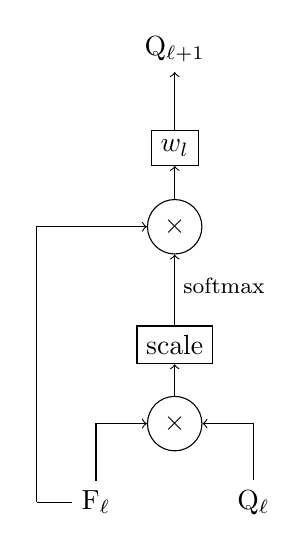
\begin{tikzpicture}
        \node (Q) at (4.5, -0.5) {Q$_\ell$};
        % \node (dimq) at (5, 0) {\scriptsize${1\times d_\ell}$};
        \node (F) at (2.5, -0.5) {F$_{\ell}$};
        % \node (dimft) at (3.0, -0) {\scriptsize${d_{\ell}\times p}$};
        \node (empt1) at (1.75, -0.5) {};
        \node[shape=circle,draw=black] (mm1) at (3.5, 0.5) {$\times$};
        % \node (dimraw) at (4,1) {\scriptsize$1\times p$};
        \node[shape=rectangle,draw=black](scale) at (3.5, 1.5) {scale};
        % \node (dimf) at (2.5, 3.175) {\scriptsize${p\times d_{\ell}}$};
        \node (soft) at (4.125, 2.25) {\footnotesize softmax};
        \node[shape=circle,draw=black] (mm2) at (3.5, 3) {$\times$};
        % \node[shape=rectangle,draw=black](project) at (3.5, 4) {$w_l: d_\ell\times d_{\ell+1}$ };
        \node[shape=rectangle,draw=black](project) at (3.5, 4) {$w_l$};
        % \node (dimscaled) [] at (4.25, 3.5) {\scriptsize $1\times d_\ell$};
        % \node [shape=circle,draw=black](sum1) at (3.5, 4) {+};
        % \node [shape=rectangle,draw=black](norm) at (3.5, 5.75) {LayerNorm};
        \node (Qplus1) at (3.5, 5.25) {Q$_{\ell+1}$};
        % \node (dimql) [align=left] at (4.25, 4.75) {\scriptsize$1\times d_{\ell+1}$};
        % \node (empt2) at (5.75, -0.5) {};
        
        \draw[->] (Q) |- node {} (mm1);
        \draw[->] (F) |- node {} (mm1);
        % \draw[-] (Q) -| node {} (empt2);
        % \draw[->] (empt2.center) |- node {} (sum1);
        \draw[->] (mm1) -- node {} (scale);
        \draw[->] (scale) -- node {} (mm2);
        \draw[-] (F) -| node {} (empt1.center);
        \draw[->] (empt1.center) |- node {} (mm2);
        \draw[->] (mm2) -- node {} (project);
        % \draw[->] (sum1) -- node {} (project);
        \draw[->] (project) -- node {} (Qplus1);
        % \draw[->] (norm) -- node {} (Qplus1);
    \end{tikzpicture}
    \caption{A Cross Attention Block. We denote matrix multiplication as "$\otimes$". The softmax operation is performed on each row). For a given layer $\ell$ we update our [CLS] token $Q_\ell$; by computing its scaled cross attention with the feature maps $F_\ell$, that are then projected to the channel dimension in the following stage, using a dense layer parametrized by $w_\ell$.}
    \label{fig:fig_crossatt}
\end{figure}

\subsection{Variations}
\label{subsec:variations}
Next we describe several versions of the Cross Attention Block.\\
\begin{figure*}[t]
    \centering
    \begin{tikzpicture}[font={\tiny},]   
         %% CNN branch
        \node(input) at (-5.5, 0) {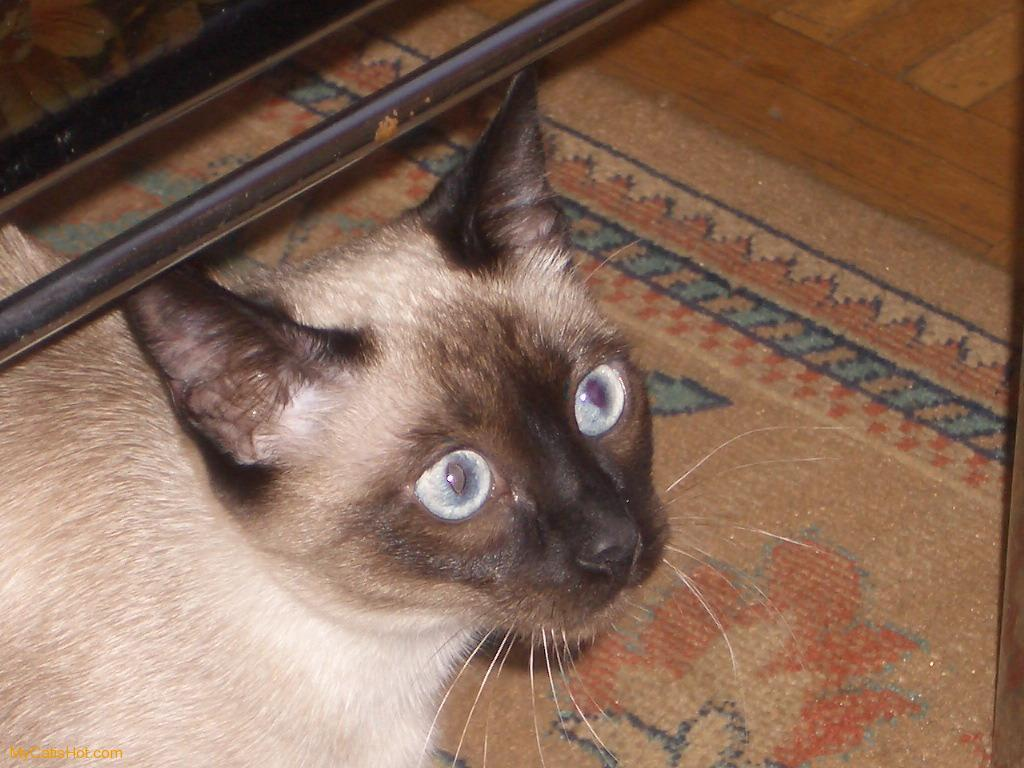
\includegraphics[width=.1\textwidth]{Images/Method/input.jpg}};
        \node[] at (input.north) {\footnotesize Input image $\vx$};
        \node[draw, trapezium, rotate=-90,trapezium angle=75, align=center] (res0) at (-3.5,0) {\rotatebox{90}{\parbox{1.0cm}{\centering{\footnotesize Res-0}\\$d_\ell:$\\64}}};
        \node[draw, trapezium, rotate=-90,trapezium angle=75, align=center] (res1) at (-1.5,0) {\rotatebox{90}{\parbox{1.0cm}{\centering{\footnotesize Res-1}\\$d_\ell:$\\64*BE}}};
        \node[draw, trapezium, rotate=-90,trapezium angle=75, align=center] (res2) at (0.5,0) {\rotatebox{90}{\parbox{1.0cm}{\centering{\footnotesize Res-2}\\$d_\ell:$\\128*BE}}};
        \node[draw, trapezium, rotate=-90,trapezium angle=75, align=center] (res3) at (2.5,0) {\rotatebox{90}{\parbox{1.0cm}{\centering{\footnotesize Res-3}\\$d_\ell:$\\256*BE}}};
        \node[draw, trapezium, rotate=-90,trapezium angle=75, align=center] (res4) at (4.5,0) {\rotatebox{90}{\parbox{1.0cm}{\centering{\footnotesize Res-4}\\$d_\ell:$\\512*BE}}};
        \node[](empt1) at (6.5, 0){};
        \node[draw, rotate=90, align=center] (class) at (7,0) {\footnotesize Classifier};
        \node(logit) at (7.75, 0) {\small$\vy$};
        %%% CLS stream
        \node[align=center](clsin) at (-4, -1.5) {{\footnotesize[CLS],}\\$d_\ell: 64$};
        \node[draw, align=center](CA0) at (-2.5, -1.5) {{\footnotesize CA-0}, \\$d_\ell:$\\64*BE};
        \node[draw, align=center](CA1) at (-0.5, -1.5) {{\footnotesize CA-1}, \\$d_\ell:$\\128*BE};
        \node[draw, align=center](CA2) at (1.5, -1.5) {{\footnotesize CA-2}, \\$d_\ell:$\\256*BE};
        \node[draw, align=center](CA3) at (3.5, -1.5) {{\footnotesize CA-3}, \\$d_\ell:$\\512*BE};
        \node[draw, align=center](CA4) at (5.5, -1.5) {{\footnotesize CA-4}, \\$d_\ell:$\\512*BE};

        %% CNN backbone
        \node(empt0) at (-4.65, 0) {};
        \draw[->] (empt0.center) -- node {} (res0);
        \draw[->] (res0) -- node {} (res1);
        \draw[->] (res1) -- node {} (res2);
        \draw[->] (res2) -- node {} (res3);
        \draw[->] (res3) -- node {} (res4);
        \draw[->] (res1) -- node {} (res2);
        \draw[->] (res2) -- node {} (res3);
        \draw[->] (res3) -- node {} (res4);
        \draw[->, blue, dashed] (res4) -- node {\blue{\normalsize//}} (class);
        \node[](GAP) at (6,0.25) {\footnotesize\blue{$\gap$}};
        \draw[->] (class) -- node {} (logit);
        %% CLS Stream
        \draw[->] (clsin) -- node {} (CA0);
        \draw[dashed, ->] (res0.north) -|node {} (CA0);
        \draw[->] (CA0) -- node {} (CA1);
        \draw[dashed, ->] (res1.north) -|node {} (CA1);
        \draw[->] (CA1) -- node {} (CA2);
        \draw[dashed, ->] (res2.north) -|node {} (CA2);
        \draw[->] (CA2) -- node {} (CA3);
        \draw[dashed, ->] (res3.north) -|node {} (CA3);
        \draw[->] (CA3) -- node {} (CA4);
        \draw[dashed, ->] (res4.north) -|node {} (CA4);
        \draw[-] (CA4.east) -| node {} (empt1.center);
        \draw[->] (empt1.center) -- node {} (class);        
        % \path[->] (CA4.east) edge[bend right,left] node {} (class.north);
        % \path [->] (B) edge[bend right=60] node {$1$} (E); 
    \end{tikzpicture}
    \caption{Cross Attention Stream applied to ResNet-based architectures. Given a CNN backbone $f(\cdot)$, we replace global average pooling with  the introduction of a global representation [CLS] learned with the inclusion of the cross attention attention stream.}
    \label{fig:fig_method}
\end{figure*}

\noindent\textbf{Cross Attention with MLP}
Regarding the architecture of transformers, we observe that following attention operation and the following projection, a feedforward network or MLP is used to further update the representation produced. To this end, we consider:\\
\begin{equation}
    \mbox{MLP}(x) = GELU(xW_1+b_1)W_2+b_2
\end{equation}
Where we maintain input and output dimensions, while the inner layer presents dimension $d_{inner} = d_l\times 2$.\\

\noindent\textbf{Projected Cross Attention}
On the operational level, our Cross Attention Block leverages the interactions between the [CLS] token and the features of a given model for a given layer \textit{l}, projecting to the dimension at the following stage \textit{l+1}. It is however possible to preserve the space in which this token lies, by the projection of the features at a given layer to the dimension of [CLS]
\begin{equation}
    \mbox{CA}_\ell(Q, F_{\ell}) = \mbox{softmax}(\frac{Q_{\ell}(F_{\ell}W^K)^\top}{\sqrt{d_Q}})F_{\ell}W^V
\end{equation}
Where the projections are parameter matrices $W^K, W^V \in \mathbb{R}^{d_\ell\times d_Q}$.

Based on these modifications for the Cross-Attention Block, we opt to keep our approach as simple as possible by using the base approach without extra projections nor MLP; nevertheless, we demonstrate the differences in performance when we choose any of the proposed variations of the self attention, as shown on Table \ref{tab:CA_variations}
 
\subsection{CLS Stream}
\noindent Taking into consideration this proposed attention module, we observe that it can be applied at different blocks of \textit{f}. In particular, we focus on depths where critical operations take place for a given network (\ie in between residual layers for ResNet architectures). Conversely, ever since its proposal GAP has been used to rely information from feature maps into the classifier stages for CNNs; however since this pooling approach is uniform, the contribution of relevant image patches towards classification is reduced. To alleviate this, we utilize our {[class]} token to update the representation examined at earlier points in the model, while also pooling the features found in the latest convolutional block of \textit{f}. An example of this stream can be observed in Figure \ref{fig:fig_method} where it is applied to a ResNet based architecture.
%Taking into consideration this proposed attention module, we observe that it can be applied at different blocks of \textit{f}. In particular, we focus on depths where changes in the area of feature maps gets reduced by pooling operations. Conversely, ever since its proposal GAP has been used to rely information from feature maps into the classifier stages for CNNs; however since this pooling approach is uniform, the contribution of relevant image patches towards classification is reduced. To alleviate this, we utilize our {[class]} token to update the representation examined at earlier points in the model, while also pooling the features found in the latest convolutional block of \textit{f}. An example of this stream can be observed in Figure \ref{fig:fig_method} where it is applied to a ResNet based architecture. 


%% To do: v3 without FC and Matrix V3 FC, no FC